\begin{figure}[htb]
    \centering
    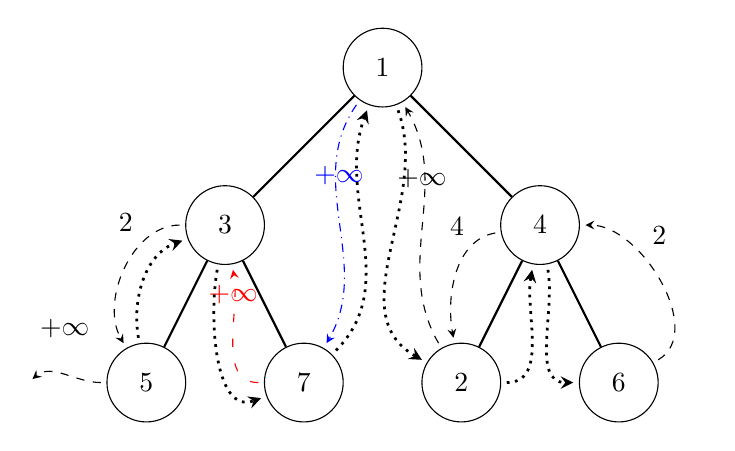
\begin{tikzpicture}[baseline=-2.25cm]
        \node[circle,draw,minimum size=1cm] (1) at (0,0)  {$1$};
        \node[circle,draw,minimum size=1cm] (2) at (-2,-2){$3$};
        \node[circle,draw,minimum size=1cm] (3) at (2,-2) {$4$};
        \node[circle,draw,minimum size=1cm] (4) at (-3,-4){$5$};
        \node[circle,draw,minimum size=1cm] (5) at (1,-4) {$2$};
        \node[circle,draw,minimum size=1cm] (6) at (3,-4) {$6$};
        \node[circle,draw,minimum size=1cm] (7) at (-1,-4){$7$};
        % \node[label={7},circle,draw,minimum size=1cm] (7) at (3,-4) {$8$};
        % \node[label={9},circle,draw,minimum size=1cm] (9) at (-2,-6) {$1$};
        \tikzstyle{filho}=[thick]
        \tikzstyle{pred}=[->, shorten >= 2pt, shorten <= 2pt,
            dashed, >=stealth]
        \tikzstyle{sucessor}=[->, shorten >= 2pt, shorten <= 2pt,
            dotted, >=stealth, line width=0.35mm]
        % \tikzstyle{p4}=[->, shorten >= 2pt, shorten <= 2pt, dotted, >=stealth]
        \draw[filho] (1) -- (2);
        \draw[filho] (1) -- (3);
        \draw[filho] (2) -- (4);
        \draw[filho] (2) -- (7);
        \draw[filho] (3) -- (5);
        \draw[filho] (3) -- (6);
        \draw[pred] (6) edge[out=30,in=0]
            node[above=10pt] {$2$} (3);
        \draw[sucessor] (3) edge[out=280,in=180] (6);
        \draw[pred] (3) edge[out=190,in=100]
            node[above=10pt] {$4$} (5);
        \draw[sucessor] (5) edge[out=0,in=260] (3);
        \draw[pred] (5) edge[out=120,in=300]
            node[above=10pt] {$+\infty$} (1);
        \draw[sucessor] (1) edge[out=290,in=150] (5);
        \draw[pred, loosely dashed, red] (7) edge[out=180,in=280]
            node[red, above=10pt] {$+\infty$} (2);
        \draw[sucessor] (2) edge[out=260,in=200] (7);
        \draw[pred, blue, dashdotted] (1) edge[out=235,in=60]
            node[blue, above=10pt] {$+\infty$} (7);
        \draw[sucessor] (7) edge[out=45,in=250] (1);
        \draw[pred] (2) edge[out=180,in=120]
            node[above=10pt] {$2$} (4);
        \draw[sucessor] (4) edge[out=100,in=200] (2);
        \draw[pred] (4) edge[out=180,in=40]
            node[above=10pt] {$+\infty$} (-4.5, -4);
    \end{tikzpicture}
    \begin{tabular}{|c|c|c|c|c|}
        \hline
         & & & $\now = 1$ \\
        $i$ & $x_0$ & $v$ & $\cert[i]$ \\
        \hline
        $1$ & $6$ & $2$ & \textcolor{blue}{$+\infty$} \\

        $2$ & $3$ & $5$ & $+\infty$ \\

        $3$ & $2$ & $1$ & $2$ \\

        $4$ & $7$ & $4$ & $4$ \\

        $5$ & $-2$ & $3$ & $+\infty$ \\

        $6$ & $14$ & $0.5$ & $2$ \\

        $7$ & $3$ & $1$ & \textcolor{red}{$+\infty$} \\
        \hline
    \end{tabular}
    \caption[ABB após chamar \textsc{insert}]{Após chamar
    \textsc{insert}$(1, 4)$, no instante $1$, o elemento $7$ foi
    inserido na árvore. O certificado do elemento $7$ foi criado e o
    certificado do seu sucessor, o elemento $1$, atualizado.}
    \label{fig:abb:insert}
\end{figure}